\subsubsection{Primera interacción con la aplicación dentro de la sala de clases}

{\textbf {Resumen:}}
El usuario (alumno enseñanza media) luego de que su profesor le hiciera entrega de una guía con la imagen QR de uno de los museos, descarga la aplicación indicada en esta, al terminar de descargar la app, la inicia, activa la cámara y apunta a la imagen con ella, al hacer esto el usuario visualiza sobre la imagen como se dibuja la habitación de un museo y ve en las indicaciones en pantalla, este se da cuenta de que puede explorar en la habitación para encontrar las piezas que esté muestra las cuales están escondidas dentro de este entorno. Además prueba las diferentes acciones para desplazarse por el museo. Luego al encontrar una pieza el usuario presiona sobre ella y descubre que ha encontrado un objeto, el cual es añadido a su colección de piezas, el usuario entusiasmado voltea a mostrarle a sus compañeros el descubrimiento.

{\textbf {Actores:}}
Alumno enseñanza media, Profesor.

{\textbf {Propósito:}}
Introducir al alumno el aprendizaje del museo local en cuestión, el cual se encuentra presente en la guía entregada por el profesor.

{\textbf {Tipo:}}
Primario.

{\textbf {Referencias cruzadas:}}
R 1.1, R 1.2, R 1.3, R 2.1, R 2.2, R 2.7, R 3.4, R 5.9.

\paragraph{Caso de Uso Esencial}

\begin{longtable}{|p{5cm}|p{8cm}|}
\hline 
Acción actores & Respuesta del sistema \\ 
\hline 
XXXX & XXXX \\ 
\hline 
\end{longtable}

\paragraph{Diagrama de Caso de Uso}

\begin{figure}[H]
\centerline{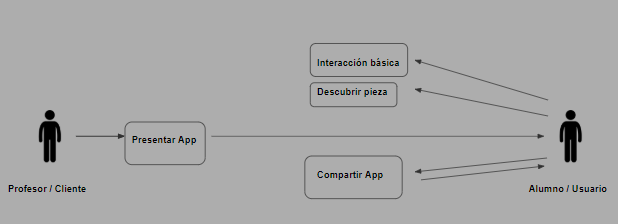
\includegraphics[width=15cm]{imgs/CasoUso_1.PNG}}
\caption{Caso-1}
\label{fig}
\end{figure}

\paragraph{Modelo Conceptual}

\begin{figure}[H]
\centerline{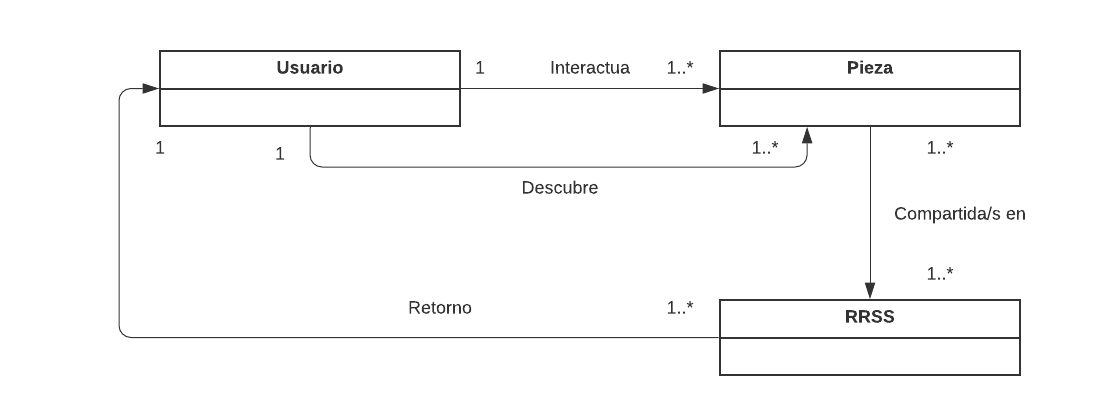
\includegraphics[width=15cm]{imgs/ModeloConceptualCaso_1_3.png}}
\caption{Caso-1}
\label{fig}
\end{figure}

\paragraph{Diagrama de Secuencia o Colaboración}

\begin{figure}[H]
\centerline{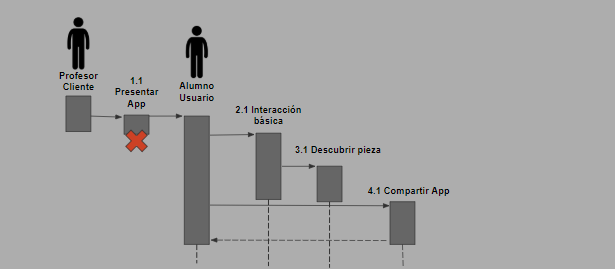
\includegraphics[width=15cm]{imgs/CasoUso_1_2.PNG}}
\caption{Caso-1}
\label{fig}
\end{figure}

\subsubsection{Priorización}
{\textbf {Tipo:}}
Primario.